\documentclass[12pt]{article}

\parskip 1ex plus 0.4ex minus 0.4ex
\parindent0ex

\usepackage{enumerate}
\usepackage{prettyref}
\usepackage{pdfpages}
\usepackage{float}
\usepackage{dirtree}
\usepackage{xltxtra}
\usepackage{polyglossia}
\setdefaultlanguage[spelling=new]{german}
\usepackage{fontspec}
\usepackage{listings}
\usepackage{xcolor}
\usepackage{amsmath}
\usepackage{amsthm}
\usepackage{amstext}
\usepackage{amssymb}
\usepackage{graphicx}
\usepackage[colorlinks,
pdfpagelabels,
pdfstartview = FitH,
bookmarksopen = true,
bookmarksnumbered = true,
linkcolor = blue, %Farbe
plainpages = false,
hypertexnames = false,
citecolor = black,
xetex] {hyperref}
\usepackage[style=alphabetic,backend=biber]{biblatex}
\bibliography{bib}

\title{Praktikumsbericht: Buffer Overflow}
\author{Marcus Ganske, 36603\\
		Lukas Krieg, 53506}
\date{\today}

\definecolor{light-gray}{gray}{0.95}

\lstset{
	language=python,
	breaklines,
	basicstyle=\ttfamily\small,
	backgroundcolor=\color{light-gray},
	keywordstyle=\color{blue},
	stringstyle=\color{olive},
	commentstyle=\color{gray}\ttfamily,
	numbers = left,
	numberstyle = \tiny,
	numberblanklines=true,
	stepnumber = 1,
	tabsize = 4,
	numbersep=10pt,
	xleftmargin=10pt,
}

\begin{document}
\maketitle
\vspace{+8cm}{
}

\includegraphics[width=12cm]{Hochschule-aalen.pdf}

\newpage
%Inhaltsverzeichnis
\renewcommand\contentsname{Inhaltsverzeichnis}
\tableofcontents
\newpage


\newpage
<<<<<<< HEAD
	\section{Aufgabe 1: Codeanalyse \& Reverse Engineering}
		In diesem Kapitel wird auf Aufgabe 1 des Praktikums eingegangen.
		Es sollte der folgende Code implementiert und analysiert werden.
		\lstinputlisting{../code/unistd.c}

		Der Quellcode des C Programms wurde in der Datei unistd.c implementiert.
		Diese Datei befindet sich im verzeichnis Code

\subsection{Codeanalyse}
\textbf{Beschreiben sie die Funktionsweise des Codes}\\
Das C-Programm initialisiert in Zeile 3 ein String Array mit Variablennamen cmd. 
Der Inhalt der Strings ist: \\
\begin{lstlisting}
"/bin/sh"
"-c"
"ls -l"
(char *)0 // NULL Pointer Value von Typ char.
\end{lstlisting}
Danach wird in Zeile 4 ein Integer mit Variablennamen "ret" definiert.\\
Die Funktion execve wird aufgerufen mit den \"Ubergabeparametern.
\begin{lstlisting}
>>>>>>> 716d1612e53e9b514228f3daf373822dd1ea1c53
cmd[0] 	-> "/bin/sh"
cmd		-> "/bin/sh", "-c", "ls -l", NULL Pointer Value
NULL
			\end{lstlisting}

			\paragraph{Funktionsaufruf execve}
			~\\
			Die Funktion Execve f\"uhrt Programme aus, auf welche mit einem Dateipfad gezeigt wird.\\
			In diesem Fall handelt es sich um den ersten \"Ubergabeparameter cmd[0]
			worin sich der Pfad "/bin/sh" befindet. Es wird eine Shell gestartet.

<<<<<<< HEAD
			Der zweite \"Ubergabeparameter von execve muss ein Array aus Argumentstrings sein, die an das neue Programm \"ubergeben werden. In diesem Fall:

			\begin{lstlisting}
cmd = {"/bin/sh", "-c", "ls -l", (char*)0}
			\end{lstlisting}
			\begin{itemize}
			\item das erste Argument "/bin/sh" gibt den Interpreter an\\
			\item das zweite Argument "-c" bedeutet, dass der folgende Befehl ausgef\"uhrt werden soll\\
			\item das dritte Argument "ls -l" wird durch die Option "-c" ausgef\"uhrt\\
			\item das vierte Argument (char*) 0 ist ein Nullpointer, der ben\"otigt wird um das Ende des Arrays f\"ur execve ersichtlich zu machen
			\end{itemize}
			~\\[0.3cm]
=======
Die Funktion execve() führt Programme aus, auf welche mit einem Dateipfad gezeigt wird.
In diesem Fall handelt es sich um das erste Übergabeparameter cmd[0]
worin sich der Pfad "/bin/sh" befindet. Es wird eine Shell gestartet.
>>>>>>> 716d1612e53e9b514228f3daf373822dd1ea1c53

			Der dritte \"Ubergabeparameter von execve ist "NULL". Hier wird ein Chararray mit zus\"atzlichen Variablen erwartet, die an
das neue Programm weitergereicht werden k\"onnen. Dieser Parameter ist genau wie der zweite nullterminiert. Deswegen wird hier einfach NULL \"ubergeben.\\[0.3cm]

<<<<<<< HEAD

			Der Returnwert wird in die Integervariable "ret" geschrieben. Bei Erfolg gibt es bei execve keinen R\"uckgabewert, im Fehlerfall wird -1 zur\"uckgegeben.

		
\subsection{Reverse Engineering mit gdb}

\subsubsection{Wie werden die Übergabeparameter an die Funktion execve()
übergeben?}
Die Übergabeparameter werden in die Register 
rdx,rdi,rsi gespeichert

\begin{figure}[h!]
	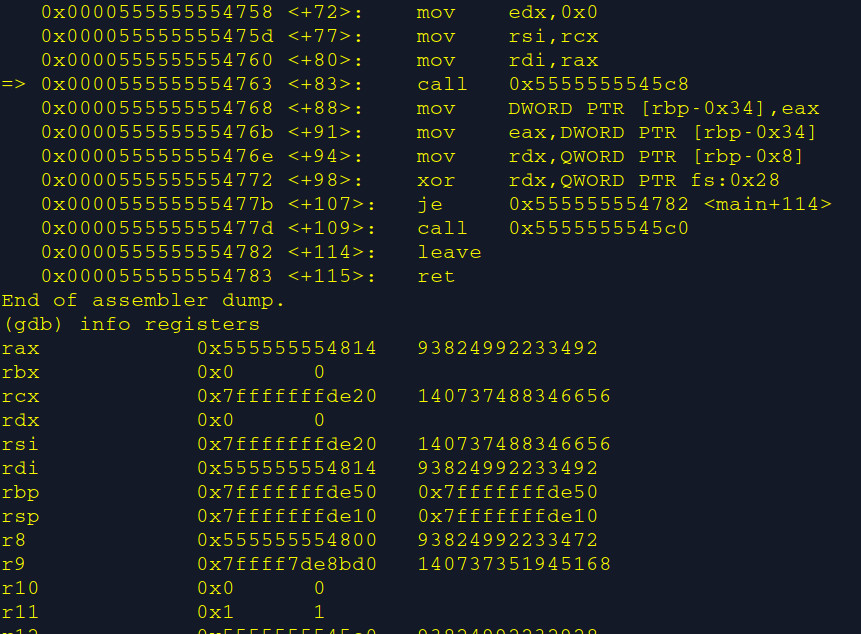
\includegraphics[width=15cm]{../images/Bufferoverflow_Aufgabe1a_Reg_b4_call.jpg}
	\caption{Aufgabe 1a Inhalt Register vor Call Execve()}
\end{figure}


\newpage

Im Register rdi befindet sich durch 
Zeile 
\begin{lstlisting}
0x0000555555554760 <+80>:   mov rdi, rax
\end{lstlisting}
die Adresse 0x555555554814 in der sich der String "/bin/sh" befindet. (siehe Abbildung 4)
\begin{lstlisting}
0x000055555555475d <+77>:   mov rsi, rcx
\end{lstlisting} 

>>>>>>> 716d1612e53e9b514228f3daf373822dd1ea1c53

Im Register rsi befindet sich die Adresse
des ersten Strings unserers Stringarrays cmd.
Die Adresse lautet 0x7fffffffde20. 
Diese Adresse liegt im Stack. 
Der Stack sieht vor dem Aufruf der Funktion folgendermaßen aus.

<<<<<<< HEAD
Die auf  0x7fffffffde20 folgenden Adressen enthalten die ben\"otigten Strings
0x7fffffffde20: 0x555555554814  -> "/bin/sh"
0x7fffffffde28: 0x55555555481c	-> "-c"
0x7fffffffde30: 0x55555555481f	-> "ls -l"
0x7fffffffde38: 0x0		-> 0
somit wird \"uber den register rsi die Variable cmd \"ubergeben.
mov eax, 0x0 
ein NULL, welches das dritte \"ubergabeparameter 
von execve ist.
=======
\begin{figure}[h!]
	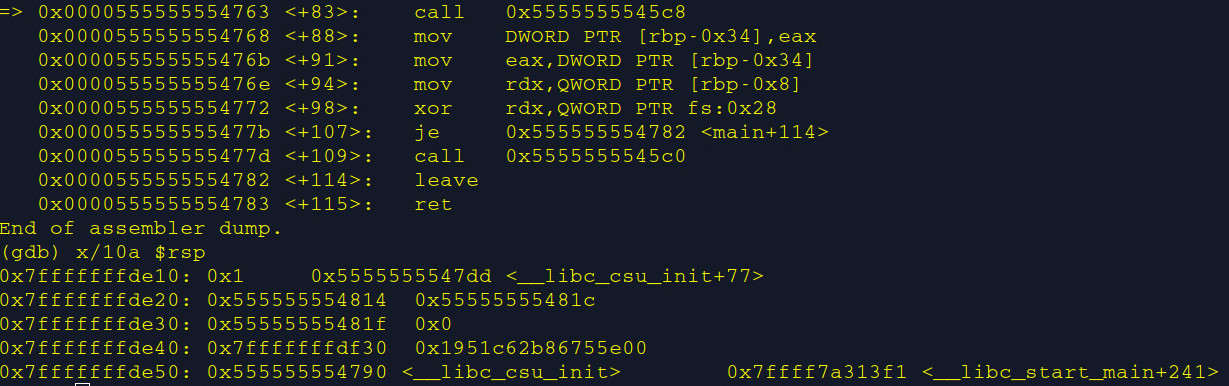
\includegraphics[width=15cm]{../images/Bufferoverflow_Aufgabe1a_StackVorCallExecve.jpg}
	\caption{Aufgabe 1a Inhalt Stack vor Aufruf execve()}
\end{figure}



\begin{lstlisting}
0x7fffffffde20: 0x555555554814  -> "/bin/sh"
0x7fffffffde28: 0x55555555481c	-> "-c"
0x7fffffffde30: 0x55555555481f	-> "ls -l"
0x7fffffffde38: 0x0
\end{lstlisting}
\begin{figure}[h!]
	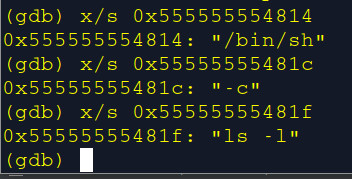
\includegraphics[width=5cm]{../images/Bufferoverflow_Aufgabe1a_Pointeruebergabeparams.jpg}
	\caption{Speicherort der Strings}
\end{figure}
Somit wird über den Register rsi das Stringarrays cmd übergeben.

\newpage
\begin{lstlisting}
0x0000555555554758 <+72>:    mov eax, 0x0 
\end{lstlisting}
Ist ein NULL, welches das dritte Übergabeparameter von execve ist.


>>>>>>> 716d1612e53e9b514228f3daf373822dd1ea1c53


\subsubsection{Wie und an welcher Stelle werden die übergebenen Parameter im Speicher abgelegt?}

Zunächst werden Pointer für alle Strings auf den Stack geschrieben um dann vor Funktionsaufruf in den entsprechenden Registern gespeichert zu werden.

<<<<<<< HEAD
ii) Wie und an welcher Stelle werden die \"ubergebenen Parameter im Speicher abgelegt?
=======
>>>>>>> 716d1612e53e9b514228f3daf373822dd1ea1c53
Dump of assembler code for function main:
\begin{lstlisting}
   0x0000555555554710 <+0>:	push rbp
   0x0000555555554711 <+1>:	mov  rbp,rsp
   0x0000555555554714 <+4>:	sub  rsp,0x40
   0x0000555555554718 <+8>:	mov  rax,QWORD PTR fs:0x28
   0x0000555555554721 <+17>:mov  QWORD PTR [rbp-0x8],rax
   0x0000555555554725 <+21>:xor  eax,eax
   0x0000555555554727 <+23>:lea  rax,[rip+0xe6]
   0x000055555555472e <+30>:mov  QWORD PTR [rbp-0x30],rax
   0x0000555555554732 <+34>:lea  rax,[rip+0xe3]
   0x0000555555554739 <+41>:mov  QWORD PTR [rbp-0x28],rax
   0x000055555555473d <+45>:lea  rax,[rip+0xdb]
   0x0000555555554744 <+52>:mov  QWORD PTR [rbp-0x20],rax
   0x0000555555554748 <+56>:mov  QWORD PTR [rbp-0x18],0x0
   0x0000555555554750 <+64>:mov  rax,QWORD PTR [rbp-0x30]
   0x0000555555554754 <+68>:lea  rcx,[rbp-0x30]
   0x0000555555554758 <+72>:mov  edx,0x0
   0x000055555555475d <+77>:mov  rsi,rcx
   0x0000555555554760 <+80>:mov  rdi,rax
   0x0000555555554763 <+83>:call 0x5555555545c8
   0x0000555555554768 <+88>:mov  DWORD PTR [rbp-0x34],eax
   0x000055555555476b <+91>:mov  eax,DWORD PTR [rbp-0x34]
   0x000055555555476e <+94>:mov  rdx,QWORD PTR [rbp-0x8]
   0x0000555555554772 <+98>:xor  rdx,QWORD PTR fs:0x28
   0x000055555555477b <+107>:je 0x555555554782 <main+114>
   0x000055555555477d <+109>:call 0x5555555545c0
   0x0000555555554782 <+114>:leave  
   0x0000555555554783 <+115>:ret  
\end{lstlisting}
\newpage
Siehe Abbildung 3 für den Inhalt des Stacks, dieser reicht von der Adresse des Registers rbp(0x7fffffffde50) bis rsp(0x7fffffffde10)
+23 Pointer von "/bin/sh" wird in Register rax geschrieben \\
+30 Pointer von "/bin/sh" wird aus rax auf den Stack Addr: rbp-0x30 geschrieben\\
+34 Pointer von "-c" wird in rax geschrieben\\
+41 Pointer von "-c" wird aus Register rax auf den Stack Addr: rbp-0x28 geschrieben\\
+45 Pointer von "ls -l" wird in Register rax geschrieben\\
+52 Pointer von "ls -l" wird aus Register rax auf den Stack Addr: rbp-0x20 geschrieben\\
+56 Die folgenden 8 Byte auf dem Stack werden mit 0 beschrieben.\\
+64 Der Pointer auf den String "/bin/sh" wird aus dem Stack in den Register rax geschrieben.\\
+68 Die Adresse rbp-0x30 wird in den rsi geschrieben, diese Adresse zeigt auf den Stack und somit auf den Begin des Stringarrays.\\
+72	0 wird in Register rdx gespeichert.\\
+77 Pointer der auf den Beginn des Stringarrays im Stack zeigt wird in rsi gespeichert.\\ 
+80 Pointer auf den String "bin/sh" wird in Register rdi gespeichert.\\

Im Stack werden die Stringadressen als QWORD Pointer gespeichert, d.h 8byte pointer =64bit

<<<<<<< HEAD
Danach werden die Parameter wie oben beschrieben aus dem Stack wieder in Register geschrieben 
um nach dem Funktionsaufruf verwendet werden zu k\"onnen.


iii)
Im stack befindet sich die R\"ucksprungadresse auf die mainfunktion
=======


\newpage
\subsubsection{Welche Daten befinden sich beim Aufruf von execve() im Stack Frame?}
Im Stack befindet sich die Rücksprungadresse auf die mainfunktion

\begin{figure}[h!]
	\includegraphics[width=10cm]{../images/Bildschirmfoto_rücksprungadresseimstack.jpg}
	\caption{neuer Stackframe beim aufruf von execve()}
\end{figure}

\begin{lstlisting}
>>>>>>> 716d1612e53e9b514228f3daf373822dd1ea1c53
(gdb) x/a $rsp
0x7fffffffde08:	0x555555554768 <main+88>
\end{lstlisting}
0x555555554768
<<<<<<< HEAD
ist die adresse die der rip nach ausf\"uhren der funktion execve wieder aufnehmen muss

dies ist der wiedereintrittspunkt in der mainfunktion

0x0000555555554763 <+83>:	call   0x5555555545c8
0x0000555555554768 <+88>:	mov    DWORD PTR [rbp-0x34],eax
0x000055555555476b <+91>:	mov    eax,DWORD PTR [rbp-0x34]
0x000055555555476e <+94>:	mov    rdx,QWORD PTR [rbp-0x8]
0x0000555555554772 <+98>:	xor    rdx,QWORD PTR fs:0x28
0x000055555555477b <+107>:	je     0x555555554782 <main+114>
0x000055555555477d <+109>:	call   0x5555555545c0
0x0000555555554782 <+114>:	leave  
0x0000555555554783 <+115>:	ret    
%\end{lstlisting}
=======
ist die Adresse die der rip nach ausführen der funktion execve wieder aufnehmen muss,
dies ist der nächste Befehl nach Aufruf der Funktion execve() in der Mainfunktion
\begin{lstlisting}
0x0000555555554763 <+83>:call 0x5555555545c8
0x0000555555554768 <+88>:mov  DWORD PTR [rbp-0x34],eax
0x000055555555476b <+91>:mov  eax,DWORD PTR [rbp-0x34]
0x000055555555476e <+94>:mov  rdx,QWORD PTR [rbp-0x8]
0x0000555555554772 <+98>:xor  rdx,QWORD PTR fs:0x28
0x000055555555477b <+107>:je   0x555555554782 <main+114>
0x000055555555477d <+109>:call 0x5555555545c0
0x0000555555554782 <+114>:leave  
0x0000555555554783 <+115>:ret    
\end{lstlisting}




>>>>>>> 716d1612e53e9b514228f3daf373822dd1ea1c53

	\section{Ein interessanter Shellcode}
		\subsection{Analyse und Beschreibung des Shellcodes}
			\lstinputlisting[linerange={1-1}]{../code/shellcode.asm}
			In dieser Zeile wird bestimmt, dass mit einer 64-Bit Architektur gearbeitet wird.

			\lstinputlisting[linerange={3-4}]{../code/shellcode.asm}		
			In diesen Zeilen werden Assembler\"ubliche Vorbereituungen getroffen.
			
			\lstinputlisting[linerange={6-14}]{../code/shellcode.asm}
			Hier beginnt der eigentliche Programmcode. Zun\"achst wird das rcx Register mit sich selbst XOR-verknüpft, um es auf 0 zu setzen. Anschlie{\ss}end wird es auf den Stack gelegt. Danach wird der Wert 0x68732f6e69622fff in rcx gelegt, der die hexadezimale Codierung von /bin/sh ist.\\
			~\\
			Anschlie{\ss}end wird mit Inhalt von rcx um ein Rechtsshift um 8 vollzogen, hierbei werden implizit alle leeren Bits auf 0 gesetzt.Hierdurch wird der Inhalt in einen nullterminierten C-String umgewandelt. Abschlie{\ss}end wird das rcx Register auf den Stack gelegt und ein Zeiger auf den String im rdi Register abgelegt.
			
			\lstinputlisting[linerange={16-19}]{../code/shellcode.asm}
			In diesem Abschnitt wird zun\"achst wieder der Wert 0 auf den Stack gelegt. Zus\"atzlich wird 0x632d, was die hexadezimale Codierung von -c ist, auf den Stack gelegt. Am Ende wird ein Zeiger auf diesen im Register rbx gespeichert.
			
			\lstinputlisting[linerange={21-23}]{../code/shellcode.asm}
			Hier wird wieder zuerst das rcx Register durch xor auf 0 gesetzt und anschlie{\ss}end auf den Stack gelegt. Anschlie{\ss}end erfolgt ein Sprung zur Commandmarke, die in Zeile 38 zu finden ist.
			
			\lstinputlisting[linerange={38-40}]{../code/shellcode.asm}
			Nach dem Sprung zur Commandmarke wird direkt die Funktion execve ausgef\"uhrt. Dies erfolgt durch einen Call, wobei gleichzeitig in Zeile 40 die R\"ucksprungadresse auf den Stack gelegt wird.
			
			\lstinputlisting[linerange={25-36}]{../code/shellcode.asm}
			Hier wird zuerst die R\"ucksprungadresse vom Stack in das rdx Register geladen und achschlie{\ss}end wieder auf den Stack gelegt. Danach wird das f\"unfte Byte dieses Blocks mit einem gro{\ss]en A xor-verkn\"upft. Anschlie{\ss]end werden die Register rbx, rdi und rsp auf den Stack gelegt und ein Zeiger auf diesen Bereich in rsi gespeichert.\\
			~\\
			Als n\"achstes wird 59 in das al Register geschrieben und anschlie{\ss}end ein syscall ausgef\"uhrt, wobei 59 f\"ur execve steht. Dies sorgt daf\"ur, dass der Befehl auf den der Zeiger im rsi Register zeigt, also /bin/sh, mit den Parametern, die unter rsi zu finden sind, also -c, ls -l und 0, und der in rdx zu findenden Variablen 0 ausgef\"uhrt.\\
			Bei dieser L\"osung bleibt die gesamte Ausf\"uhrung im selben Thread, womit der Originale Thread nicht ver\"andert werden muss.
		\subsection{Shellcode \"ubersetzen}
			Um den oben beschriebenen Shellcode auszuf\"uhren muss er zuerst \"ubersetzt werden. Dies kann mit folgendem aus der Vorlesung bekannten Befehl bewerkstelligt werden:\\
			~\\
			\texttt{nasm -f bin shellcode.asm -o shellcode.bin}\\
			~\\
			Mit Hilfe des Skripts \texttt{dumpshellcode.py} kann der Maschinencode als entsprechend formatierter Hexcode ausgegeben werden, um ihn in ein anderes Pythonskript einzubinden.
			
		\subsection{Shellcode ausf\"uhren}
			Um den Shellcode auszuf\"uhren, wird nun ein Payloadskript in Python erstellt. Die Implementierung lehnt sich an das aus der Vorlesung bekannte Skript \texttt{unic0d3r-payload.py} an.\\
			~\\
			\lstinputlisting[linerange={1-2}]{../code/sp-praktikum2-ganske-krieg-aufgabe2.py}
			Zuerst wird der Pfad zum Python Compiler angegeben und die sys-Bibliothek importiert.
			
			\lstinputlisting[linerange={5-10}]{../code/sp-praktikum2-ganske-krieg-aufgabe2.py}
			Nun wird \"uberpr\"uft, ob die Anzahl der Parameter genau 2 ist. Ist das der Fall, wird die \"ubergebene Adresse gespeichert.\\
			Im Fehlerfall wird eine entsprechende Meldung ausgegeben und das Skript beendet.

			\lstinputlisting[linerange={12-17}]{../code/sp-praktikum2-ganske-krieg-aufgabe2.py}
			Im n\"achsten Schritt wird der Shellcode eingebunden, der mit dem Skript \texttt{dumpshellcode.py} ausgegeben wurde. Er kann hier fest implementiert werden, da nur \texttt{ls -l} ausgef\"uhrt werden soll.
			tte
			\lstinputlisting[linerange={19-20}]{../code/sp-praktikum2-ganske-krieg-aufgabe2.py}
			Damit der Shellcode korrekt ausgef\"uhrt wird, m\"ussen Gr\"o{\ss}e des Nopsleds und des Paddings angepasst werden.Der Nopsled wurde fest auf 60 Operationen gesetzt. Damit muss das Padding um genau diesen Wert verringert werden.\\ Es w\"aren auch andere Gr\"o{\ss}en f\"ur den Nopsled m\"oglich.\\
			~\\
			Ausgef\"uhrt wird der Shellcode \"uber das Programm \texttt{hackme}. Dieses wird gestartet mit\\
			\texttt{./hackme "\$(./sp-praktikum2-ganske-krieg-aufgabe2.py \textit{Adresse})"}
			
	\section{Ausbau des Shellcodes}
	
	Nun soll das Skript so erweitert werden, damit jedes Kommando ausgef\"uhrt werden kann anstatt nur \texttt{ls -l}.
			Um zu verstehen, was an dem Skript ver\"andert werden muss, sollte zun\"achst die Bin\"ardarstellung des Shellcodes betrachtet werden, um herauszufinden, welche der Bytes abh\"angig vom auszuf\"uhrenden Kommando sind. Am einfachsten geht das durch Einsetzen verschiedener Kommandos und nachfolgender Ausgabe durch \texttt{dumpshellcode.py}.
			
			\lstinputlisting[linerange={12-17}]{../code/sp-praktikum2-ganske-krieg-aufgabe2.py}
			Mit dieser Vorgehensweise werden schnell zwei Stellen gefunden, an denen sich der Shellcode \"andert. Zum Einen \"andern sich die letzten Bytes des Shellcodes, da sie das auszuf\"uhrende Kommando beinhalten, und zum Anderen \"andert sich ein Byte in der Mitte des Shellcodes, das die L\"ange des auszuf\"uhrenden Kommandos angibt.\\
			~\\
			Um nun ein beliebiges Kommando ausf\"uhren zu k\"onnen, muss der Shellcode entspprechend ver\"andert werden. Das in Python implementierte Skript baut das als Parameter \"ubergebene Kommando in den Shellcode ein.\\
			~\\
			\lstinputlisting[linerange={5-9}]{../code/sp-praktikum2-ganske-krieg-aufgabe3.py}
			Im ersten Schritt werden eine Adresse, die Paddingsize und das auszuf\"uhrende Kommando eingelesen und gespeichert. 
			
			\lstinputlisting[linerange={15-24}]{../code/sp-praktikum2-ganske-krieg-aufgabe3.py}
			Als n\"achstes wird das Kommando hexadezimal codiert, seine L\"ange gespeichert und der erste Teil des Shellcodes vorbereitet. 
			
			\lstinputlisting[linerange={26-26}]{../code/sp-praktikum2-ganske-krieg-aufgabe3.py}
			Nun wird die L\"ange des Kommandos in den Shellcode eingef\"ugt.
			
			\lstinputlisting[linerange={28-29}]{../code/sp-praktikum2-ganske-krieg-aufgabe3.py}
			Danach kommt wieder ein fester Teil des Shellcodes.
			
			\lstinputlisting[linerange={31-33}]{../code/sp-praktikum2-ganske-krieg-aufgabe3.py}
			Jetzt wird die Paddingsize auf Basis der L\"ange des Nopsled berechnet.
			
			\lstinputlisting[linerange={38-38}]{../code/sp-praktikum2-ganske-krieg-aufgabe3.py}
			Am Ende wird des Shellcode zusammengesetzt.\\
			~\\
			Aufgerufen werden kann das Programm mit \\
			\texttt{./hackme "\$(.sp-praktikum3-ganske-krieg-aufgabe3.py \textit{Adresse Paddingsize 'Kommando'})"}

\end{document}
